\chapter{プロダクト}

\section{アプリケーションのコンセプト}
BuLoはバスに乗り遅れたくないが,バスを効率的に使いたいひとのためのバスロケーションアプリである.
従来のバスロケーションアプリやGoogle Mapsなどの地図アプリとは異なり,バスの位置や遅延情報をリアルタイムにわかりやすく把握することができる.
また,本サービスは“ひとめぼれ”するバスロケーションアプリをめざしている.本グループは”ひとめぼれ”を以下の2つと考える.
まず1つ目にアプリのデザインに対する”ひとめぼれ”である.これはアプリを使うきっかけとなるものである.
2つ目にアプリ全体を通しての体験への”ひとめぼれ”である.これは,アプリを使い続けるきっかけになると考える.
\bunseki{下村蒔里萌}

\section{機能}
\subsection{住所を登録}
    このアプリの対象ユーザは通勤・通学にバスを利用する人であるため,自宅と職場の住所を登録する機能を搭載している.
    対象ユーザの使用するルートは変わらないことが予測できるため,最初に住所を登録をすることで2回目以降は再度住所の検索をする手間を省いている.
    図\ref{fig:feature_register}中の左から2枚目の画面では現在地の住所を表示させている.
    左から3枚目の画面では「はこだて」と入力して,それに対しての予測を表示させている.
    \begin{figure}
        \centering
        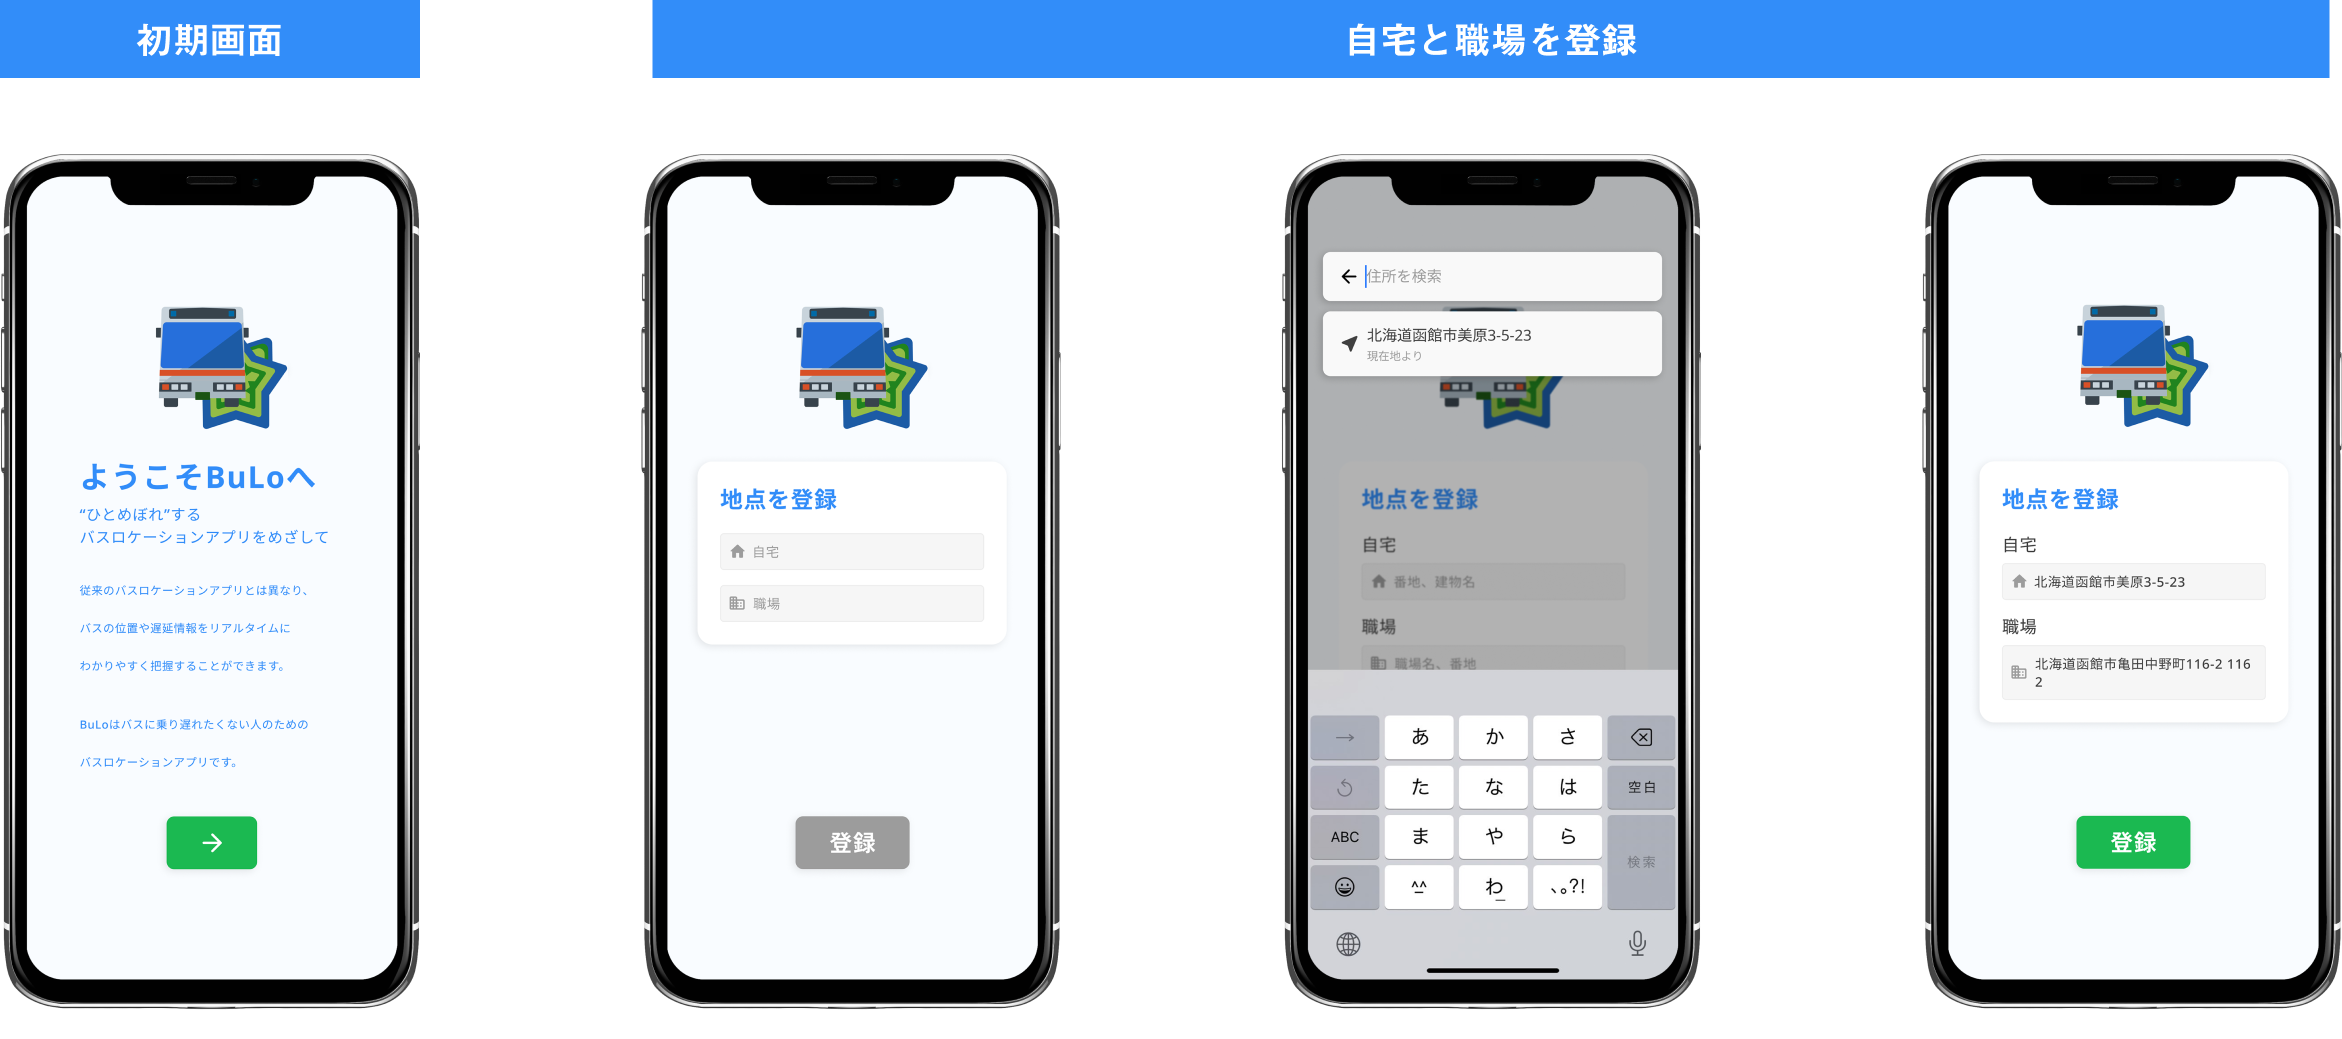
\includegraphics[width=14cm]{images/feature_register.png}
        \caption{Register View}
        \label{fig:feature_register}
    \end{figure}
\subsection{Time-Distance View}
    Time-Distance Viewとは,ユーザの現在地,バスの現在地,バス停の3点を時間的グラフに表したものである.
    これにより,ユーザは実装方法は図\label{fig:feature_timedistanceview}に示す.
    図\ref{fig:feature_timedistanceview}では以下の状況を考えている.
    \begin{figure}
        \centering
        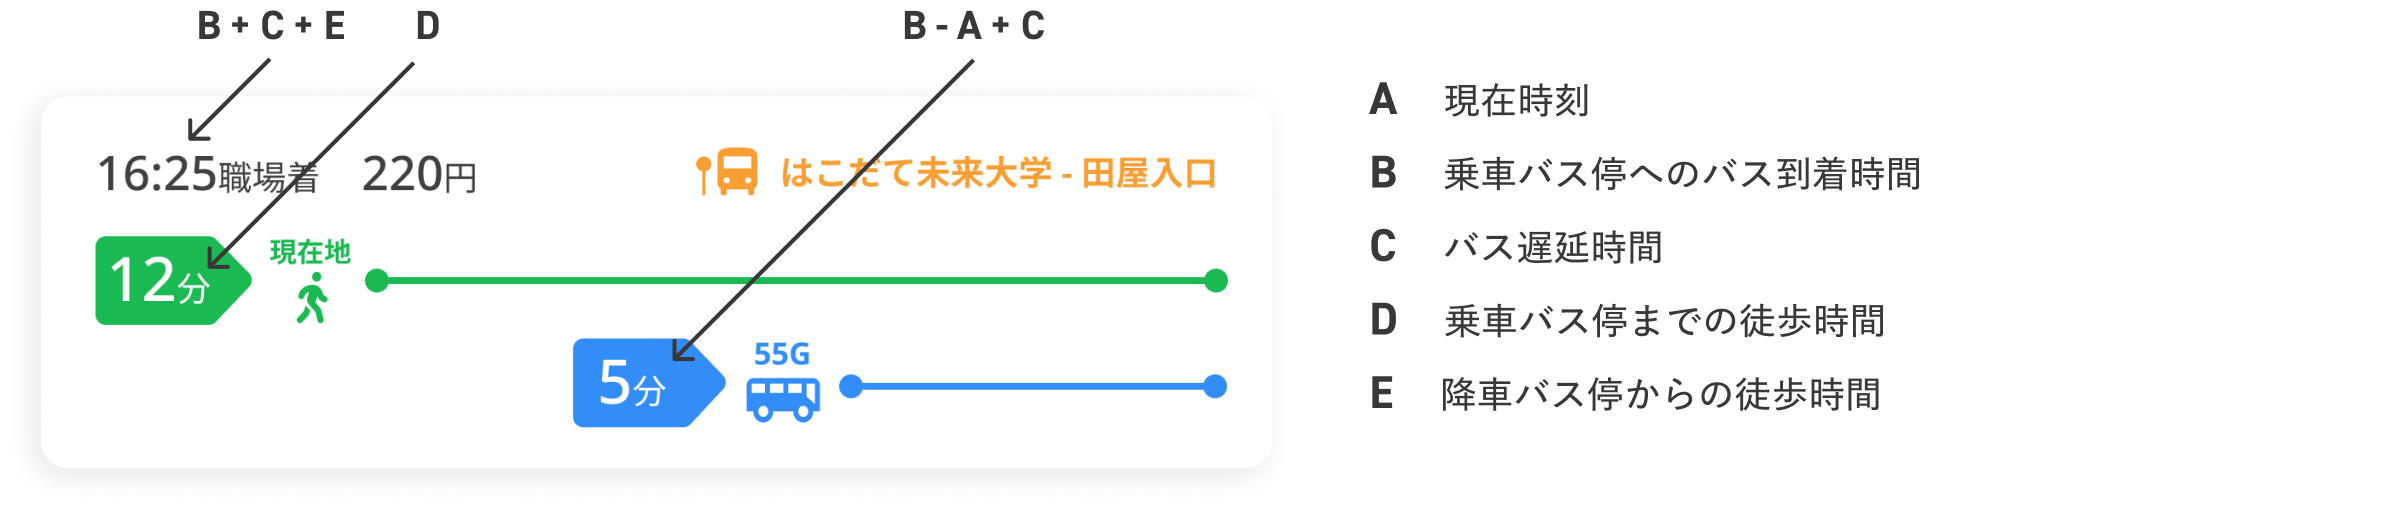
\includegraphics[width=14cm]{images/feature_timedistanceview.png}
        \caption{Time-Distance View}
        \ref{fig:feature_timedistanceview}
    \end{figure}
    \begin{quote}
        \begin{itemize}
            \item 目的地は職場
            \item 現在地からの最寄りのバス停は亀田支所前
            \item 乗るバスは55G
            \item 最寄りバス停から目的地付近のバス停までの料金は220円
            \item バスが5分後に亀田支所前に到着
            \item 亀田支所前まで歩きで3分
        \end{itemize}
    \end{quote}
\subsection{Time-Distance List}
\subsection{Route View}
\bunseki{下村蒔里萌}

\section{デザインシステム}
\bunseki{下村蒔里萌}

\section{システムの構成}
\subsection{アーキテクチャ図}
\subsection{使用した技術}